\documentclass{article}
\author{}
\usepackage{caption}
\usepackage{subcaption}
\usepackage{graphicx} %I need to include some graphs in this document
\usepackage{amsmath}
\usepackage[margin=1.2in]{geometry}

\begin{document}
\paragraph*{}
\begin{itemize}
%end{align*}
\item \mbox{08/20}
\begin{align*}
\vec{w}^2&=(\alpha\vec{r}+\beta\vec{b})^2 \\
&=\alpha^2r^2+\beta^2b^2+2\alpha\beta\vec{r}\cdot\vec{b}\\
&=\alpha^2r^2+(1-\alpha\frac{\vec{r}\cdot\vec{b}}{b^2})^2b^2+2\alpha(1-\alpha\frac{\vec{r}\cdot\vec{b}}{b^2})\vec{r}\cdot\vec{b}\\
&=\alpha^2r^2+(1+\alpha^2\frac{(\vec{r}\cdot\vec{b})^2}{b^4}-2\alpha\frac{\vec{r}\cdot\vec{b}}{b^2})b^2+2\alpha(1-\alpha\frac{\vec{r}\cdot\vec{b}}{b^2})\vec{r}\cdot\vec{b}\\
&=\alpha^2r^2+b^2-\alpha^2\frac{(\vec{r}\cdot\vec{b})^2}{b^2}\\
&=b^2+\frac{\vert\alpha\vert^2}{b^2}(r^2b^2-(\vec{r}\cdot\vec{b})^2)
\end{align*}
\item 08/26
\paragraph*{}
In our calculations, the standard deviation of temperature in a certain slab $m$ is expressed as
\begin{equation}
\sigma_{m,s}=\sqrt{\frac{\sum\limits_{i=1}^\mathcal{N}\left( T_{m,i}-\overline{T}_m\right)}{\mathcal{N}-1}}
\end{equation}
where $\overline{T}_m$ is the average value for measurements $T_{m,i}$ and $\mathcal{N}$ represents the total number of measurements.The standard deviation of the averaged value $\overline{T}_m$, therefore, is given by
\begin{align}
\sigma_m &=\frac{\sigma_{m,s}}{\sqrt{\mathcal{N}}}\\
&=\sqrt{\frac{\sum\limits_{i=1}^\mathcal{N}\left( T_{m,i}-\overline{T}_m\right)}{\mathcal{N}(\mathcal{N}-1)}}
\end{align}
\paragraph*{}
With a set of data $(\overline{T}_m,\sigma_m)$ where $m$ goes from 0 to N-1 in our model, we do the fit to the cosine function to determine and fitting parameter of amplitude, which is $\Delta T$ in Eq.(1). The standard deviation of $\Delta T$ is determined at the same time.Then by using Eq.(2) we can get a relation between $\sigma_{\Delta T}$ and $\sigma_{\kappa_{\mbox{eff}}}$, which is
\begin{equation}
\frac{\sigma_{\kappa}}{\kappa_{\mbox{eff}}}=\frac{\sigma_{\Delta T}}{\Delta T}
\end{equation}
Thus $\sigma_{\kappa_{\mbox{eff}}}=\kappa_{\mbox{eff}}\sigma_{\Delta{T}}/\Delta{T}$ gives the standard deviation of $\kappa$.
\end{itemize}
\section*{Liquid}
\section*{Crystal}
\begin{itemize}
\item \mbox{08/09}\\
Temperature approximately 80K, 0.66 in LJ unit, with the scaling $\epsilon/k_B=119.6K$, I keep the temperature variance 0.03 during the simulation(LJ unit) to keep my system efficient.We run those systems at constant temperature.
\section*{Extrapolation}
\item \mbox{08/23} correction\\
\begin{figure}[h]
    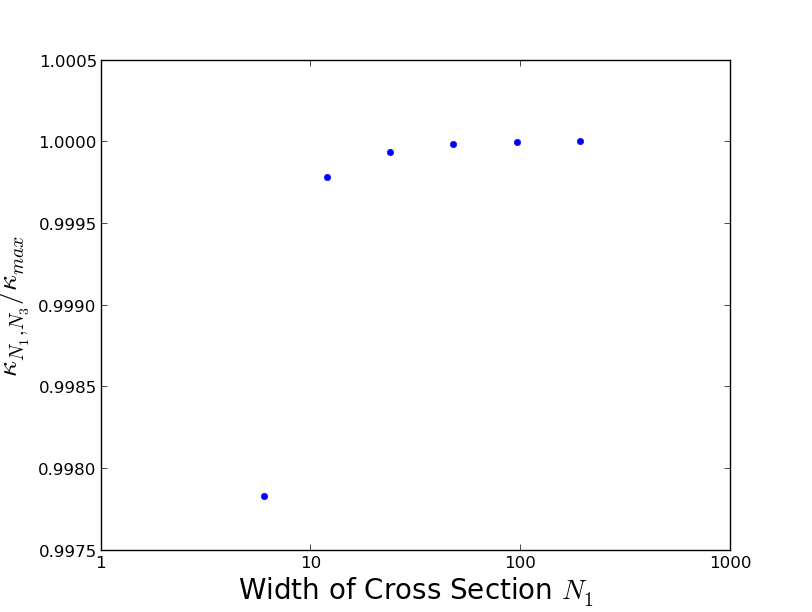
\includegraphics[height=6cm]{Cross5.png}
\end{figure}
summing over Brillouin Zone, the length of the sample is 500a=500d, the ratio is devided by the kappa(192)
\end{itemize}
\paragraph*{Appendix A}
\begin{align*}
\kappa(q)&=\frac{3\kappa_{D,0}}{7\lambda^2}[o(\lambda^3)+1+2\lambda^2-(1-\frac{1}{3}\lambda^2)-\frac{\lambda^{\frac{5}{2}}}{\sqrt{2}}(o(\sqrt{\lambda})+\pi)] \\
&=\kappa_{D,0}-\frac{3\pi\sqrt{\lambda}} {7\sqrt{2}}\kappa_{D,0}\\
&=\kappa_{D,0}-\frac{3\pi} {7}\kappa_{D,0}\sqrt{\frac{\pi \l_{min}}{L}}
\end{align*}

\paragraph*{}
Here $o(\lambda^3)$ means terms that have a order lower than or equal to $\lambda^3$ in $\lambda\longrightarrow 0$ limit, I am guessing that in summing the $\frac{1}{3}\lambda^2$, the appendix A wrongly subtracted it.

\paragraph*{Appendix B}
\begin{align*}
\frac{\kappa_{00}(q)}{\kappa_{D,0}}&= \frac{n^{\frac{1}{3}}}{2N_xN_y}\int_\epsilon^1 dx\frac{x^2}{x^4+\lambda^4}\\
&= \frac{n^{\frac{1}{3}}}{2N_xN_y}\times \frac{1}{\sqrt{\lambda}}[\frac{\sqrt{2}}{8}\ln\frac{1+\lambda+\sqrt{2\lambda}}{1+\lambda-\sqrt{2\lambda}}+\frac{\sqrt{2}}{4}\arctan(\sqrt{\frac{2}{\lambda}}+1)+\frac{\sqrt{2}}{4}\arctan(\sqrt{\frac{2}{\lambda}}-1)\\
&-\frac{\sqrt{2}}{8}\ln\frac{1+\frac{\epsilon^2}{\lambda}-\sqrt{\frac{2}{\lambda}}\epsilon}{1+\frac{\epsilon^2}{\lambda}+\sqrt{\frac{2}{\lambda}}\epsilon}-\frac{\sqrt{2}}{4}\arctan(\sqrt{\frac{2}{\lambda}}\epsilon+1)-\frac{\sqrt{2}}{4}\arctan(\sqrt{\frac{2}{\lambda}}\epsilon-1)]\\
&=\frac{n^{\frac{1}{3}}}{2N_xN_y}\times \frac{1}{\sqrt{\lambda}}(\frac{\sqrt{2}}{8}\ln\frac{1+\lambda+\sqrt{2\lambda}}{1+\lambda-\sqrt{2\lambda}}+\frac{\sqrt{2}}{4}\pi)\\
&=\frac{n^{\frac{1}{3}}}{2N_xN_y}\times \frac{1}{\sqrt{\lambda}}(-\frac{1}{2}\sqrt{\lambda}+\frac{\sqrt{2}}{4}\pi)\\
&=\frac{n^{\frac{1}{3}}}{2N_xN_y}\times(\frac{\sqrt{2}}{4}\frac{\pi}{\sqrt{\lambda}}-\frac{1}{2})\\
&=\frac{n^{\frac{1}{3}}}{2N_xN_y}\times(\frac{1}{4}\sqrt{\frac{\pi L}{\ell_m}}- \frac{1}{2})
\end{align*}

\section*{Q}
For  a crystal of a $N_1\times N_2\times N_3$ cell in the real space: \\
The wave vector we are summing over is in the form$\vec{Q}=\frac{2\pi}{a}(\frac{n_1}{N_1},\frac{n_2}{N_2},\frac{n_3}{N_3})$\\
where $n_1,N_2,n_3$ are to be decided.
\paragraph*{}
There are 8 constraints on $n_1,n_2,n_3$,because by the property of BZ, the BZ is enclosed by the bi-sector of wave vector:\\
\begin{center}
$\frac{2\pi}{a}(1,1,1),\frac{2\pi}{a}(\bar{1},\bar{1},\bar{1});\frac{2\pi}{a}(\bar{1},1,1),\frac{2\pi}{a}(1,\bar{1},\bar{1});$\\
$\frac{2\pi}{a}(1,\bar{1},1),\frac{2\pi}{a}(\bar{1},1,\bar{1})
$ and $\frac{2\pi}{a}(1,1,\bar{1}),\frac{2\pi}{a}(\bar{1},\bar{1},1);$\\
\end{center}

\paragraph*{}
For $\frac{2\pi}{a}(1,1,1),\frac{2\pi}{a}(\bar{1},\bar{1},\bar{1})$:
\begin{equation*}
-\frac{\sqrt{3}}{2}<\frac{\frac{n_1}{N_1}+\frac{n_2}{N_2}+\frac{n_3}{N_3}}{\sqrt{3}}\leq\frac{\sqrt{3}}{2}
\end{equation*}
$\Longleftrightarrow$
\begin{equation*}
-3N_1N_2N_3<2n_1N_2N_3+2N_12_2N_3+2N_1n_2N_3+2N_1N_2n_3< 3N_1N_2N_3+1
\end{equation*}
For $\frac{2\pi}{a}(\bar{1},1,1),\frac{2\pi}{a}(1,\bar{1},\bar{1})$:
\begin{equation*}
-3N_1N_2N_3<-2n_1N_2N_3+2N_12_2N_3+2N_1n_2N_3+2N_1N_2n_3< 3N_1N_2N_3+1
\end{equation*}
$(1,\bar{1},1)$, $(1,1,\bar{1})$ are similar.
\paragraph*{}
we can use a triple-loops to search these wave vectors:\\
\begin{center}
$n_1:-N_1+1\rightarrow N_1$ \\
$n_2:-N_2+1\rightarrow N_2$ \\
$n_3:-N_3+1\rightarrow N_3$ 
\end{center}

\end{document}